\section{Manual de usuario} \label{sec:manual-usuario}

\subsection{Primer uso}\label{sec:primer-uso}
Para el primer uso, es necesario tener disponible una red WiFi con los siguientes parámetros. Esto se puede conseguir utilizando un celular o una notebook, configurandola como punto de acceso, como hacer esto no se cubrirá en esta guía.

\begin{description}
	\item[Nombre de red (SSID):] TP12017G7
	\item[Contraseña de red:] abcd1234
\end{description}

El cartel tomará la IP 192.168.43.254, sin importar a qué red esté conectada.

El microcontrolador cuando se prende por primera vez, tendrá un mensaje predeterminado y se conectará a la siguiente red predefinida:

La contraseña de acceso por defecto será \enquote{1234}. Ésta deberá ser modificada rápidamente en el primer uso, para evitar que un atacante lo haga antes. Este procedimiento se explica en la sección \ref{sec:guia-password}.

Como siguiente paso, se debe cambiar la red a la que se conecta el cartel a una red WiFi fija, a la que siempre se conectará el cartel al encenderse. Este procedimiento se explica en la sección \ref{sec:guia-wifi}.

\subsection{Uso del cartel}\label{sec:guia-uso}
\subsubsection{Conexión al cartel}\label{sec:guia-conexion}
Para conectar al cartel, simplemente abra el programa. Al abrir, lo primero que aparecerá es un diálogo pidiendo la dirección (en nombre o IP) del cartel.  Se puede ver este diálogo en la figura \ref{fig:scr-login}.

\begin{figure}[ht]
	\centering
	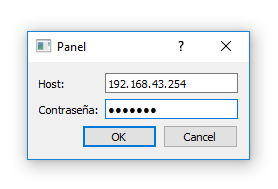
\includegraphics[scale=0.8]{imagenes/scr-login.png}
	\caption{Captura de pantalla de la ventana de login.}
	\label{fig:scr-login}
\end{figure}

Ingrese la dirección y la contraseña y haga click en \enquote{Aceptar}. Si la contraseña es correcta, será llevado a la ventana principal de la aplicación. En caso contrario, se volverá a pedir los datos hasta que sean correctos. Se puede ver una captura de pantalla de la ventana principal en la figura \ref{fig:scr-principal}

\begin{figure}[ht]
	\centering
	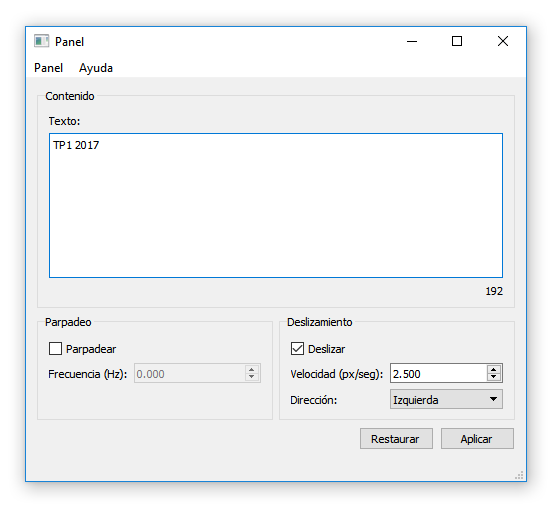
\includegraphics[scale=0.8]{imagenes/scr-principal.png}
	\caption{Captura de pantalla de la ventana principal.}
	\label{fig:scr-principal}
\end{figure}

\subsubsection{Cambio de contraseña de acceso}\label{sec:guia-password}
Para realizar esta acción se necesita haber ingresado previamente la contraseña de acceso y encontrarse en la ventana principal de la aplicación.

Haga click sobre el menú \enquote{Panel} y luego en {Cambiar contraseña...}. Esto abrirá la ventana diálogo de cambio de la contraseña, que se puede ver la figura \ref{fig:scr-passwd}.

\begin{figure}[ht]
	\centering
	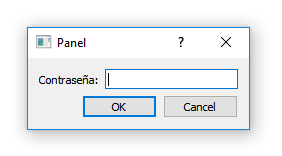
\includegraphics[scale=0.8]{imagenes/scr-passwd.png}
	\caption{Captura de pantalla de la ventana de cambio de contraseña.}
	\label{fig:scr-passwd}
\end{figure}

Una vez en esta ventana, ingrese la nueva contraseña. Ésta no deberá ser más larga que 40 caracteres.
Luego, presione \enquote{Aceptar} para realizar el cambio u \enquote{Cancelar} para cancelar.

\subsubsection{Cambio de mensaje al cartel}\label{sec:guia-texto}
Para realizar esta acción se necesita haber ingresado anteriormente la contraseña de acceso y encontrarse en la ventana principal de la aplicación.

Estando en la ventana principal de la aplicación, simplemente se debe escribir en el campo \enquote{Texto} el texto deseado. A medida que se vaya escribiendo, se indicará en la esquina inferior derecha la cantidad de caracteres restantes que se pueden escribir.

Opcionalmente se puede activar el parpadeo. Para esto haga click sobre la casilla de verificación \enquote{Parpadeo} y defina el valor de frecuencia deseado en Hertz. El mismo procedimiento aplica para la velocidad de desplazamiento.

\subsubsection{Cambio de red WiFi}\label{sec:guia-wifi}
Para realizar esta acción se necesita haber ingresado anteriormente la contraseña de acceso y encontrarse en la ventana principal de la aplicación.

Haga click sobre el menú \enquote{Panel} y luego en \enquote{Cambiar configuración de red...}. Esto abrirá un dialogo con campos editables que corresponden al nombre de red y la contraseña de la red a la cual deberá conectarse el cartel al aplicar el cambio. Se puede ver esta ventana en la figura \ref{fig:scr-wifi}.

\begin{figure}[ht]
	\centering
	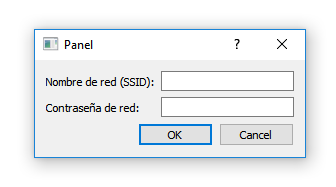
\includegraphics[scale=0.8]{imagenes/scr-wifi.png}
	\caption{Captura de pantalla de la ventana de cambio de configuración WiFi.}
	\label{fig:scr-wifi}
\end{figure}

Luego, presione \enquote{Aceptar} para realizar el cambio u \enquote{Cancelar} para cancelar.

\subsubsection{Reestablecimiento de configuración}\label{sec:guia-reset}
Para realizar esta acción se necesita acceso físico al hardware.

Puede ocurrir que la red a la cual el cartel se conecta ya no esté disponible o el administrador del cartel se haya olvidado o perdido la contraseña. En estos casos es deseable llevar el cartel a un estado conocido.

Para reestablecer la configuración del cartel, presione el botón de RESET del cartel por aproximadamente 5 segundos. Sabrá que se reinicio cuando vea parpadear el cartel y aparezca un mensaje inicial genérico. A partir de este momento, el cartel volverá a conectarse a la red especificada en la sección \ref{sec:primer-uso}.
